\documentclass[11pt]{article}

\usepackage{amsmath}
\usepackage{graphicx}
\usepackage{hyperref}
\usepackage{booktabs}
\usepackage[margin=1in]{geometry}
\usepackage{natbib}
\usepackage{microtype}
\usepackage{xcolor}
\usepackage{siunitx}
\usepackage{tabularx}

\hypersetup{
    colorlinks=true,
    linkcolor=blue,
    citecolor=blue,
    urlcolor=blue
}

\title{A 12{,}573-Residue Audit of D-Amino Acid Stereochemistry in the Protein Data Bank}
\author{Tommaso R.\ Marena\\
\textit{The Catholic University of America, Washington, DC}\\
\texttt{marena@cua.edu}}
\date{}

\begin{document}

\maketitle

\begin{abstract}
We audited 12{,}573 D-amino acid C$_\alpha$ stereocenters across 4{,}616 PDB entries --- covering $>$91\% of all RCSB entries for each of the 18 standard D-amino acid Chemical Component Dictionary (CCD) codes --- using only the signed tetrahedron volume of the four backbone substituents (N, C$_\alpha$, C, C$_\beta$). 29 D-labeled residues in 16 deposited structures show positive signed volumes, indicating L-stereochemistry at C$_\alpha$ despite the D-amino acid label (0.23\% mismatch rate). Cross-referencing against deposition metadata, COMPND records, and primary literature classifies these as: 6 genuine stereochemistry errors (biology requires D, coordinates show L), 18 CCD-code misassignments (L-form ligand with D-form CCD code), 3 polymer residue mislabels, and 2 borderlines. Errors concentrate in five CCD codes (DTY, DLY, DAR, DPN, DSN) and span 0.99--3.4~\AA\ resolution; deposition year significantly predicts errors (Mann--Whitney $U=278$, $p=0.0027$), resolution does not ($p=0.19$). MolProbity does not flag any of these. We argue these errors reflect a systematic gap in the wwPDB deposition pipeline: D-amino acid C$_\alpha$ chirality is not validated against the configuration encoded in the CCD InChI \texttt{/m} flag, and an automated check that compared signed volumes to that flag would catch every CCD misassignment reported here at deposit time.
\end{abstract}

\noindent\textbf{Keywords:} D-amino acid; chirality; PDB validation; CCD; wwPDB remediation.

\section{Introduction}

D-amino acid residues appear in the PDB in three biologically and structurally distinct contexts: as ribosomally L-encoded residues post-translationally epimerized in natural products (e.g.\ daptomycin, contryphans), as components of mirror-image-designed or NRPS-assembled therapeutic peptides, and as small-molecule ligands (substrate analogues and inhibitors) where the D-form is one of several stereoisomers available in the chemical component dictionary. Each of these contexts has independent biological constraints on configuration, but the wwPDB deposition pipeline does not check those constraints against the deposited C$_\alpha$ coordinates. MolProbity --- the de facto standard for stereochemistry validation \citep{chen2010,lovell2003} --- validates L-amino acid C$_\alpha$ chirality but does not extend the check to D-labeled residues. The 2006--2008 wwPDB remediation effort \citep{henrick2008} corrected many stereochemistry-related annotations across the archive but did not specifically address D-amino acid configuration.

We previously showed \citep{hovmoller2002} that the signed volume of the C$_\alpha$ tetrahedron is sufficient to discriminate L from D at any standard amino acid stereocenter with positive backbone atom coverage. Here we apply this check across $>$91\% of the RCSB universe of each of the 18 standard D-amino acid CCD codes to characterize the scope, structure, and remediation pathway of D-chirality annotation errors in the PDB.

\section{Methods}

\subsection{Signed Tetrahedron Volume}

For each D-labeled residue with complete backbone (N, C$_\alpha$, C, C$_\beta$), the signed volume is computed as
\begin{equation}
v = (\mathbf{N} - \mathbf{C}_\alpha) \cdot \left[ (\mathbf{C} - \mathbf{C}_\alpha) \times (\mathbf{C}_\beta - \mathbf{C}_\alpha) \right].
\end{equation}
Under the CIP convention, $v < 0$ at a correctly modeled D-residue (R-configuration) and $v > 0$ at an L-residue (S-configuration). A D-labeled residue with $v > 0$ is therefore a label/coordinate mismatch.

\subsection{Dataset Construction}

For each of the 18 standard D-amino acid CCD codes (DAL, DAR, DAS, DCY, DGL, DGN, DHI, DIL, DLE, DLY, DPN, DPR, DSG, DSN, DTH, DTR, DTY, DVA), we enumerated all RCSB entries via the official text search API and downloaded the legacy PDB-format coordinate files. 245 entries deposited exclusively as mmCIF (predominantly post-2019 large cryo-EM assemblies) were excluded; coverage statistics in Table~\ref{tab:coverage} reflect the legacy-format subset. The full per-residue dataset (raw N/C$_\alpha$/C/C$_\beta$ coordinates, signed volume, and chirality classification) is provided as \texttt{results/d\_residue\_verification.csv}.

\subsection{Independent Verification}

To eliminate ChiralFold-implementation artifacts, the audit was reproduced by an independent script (\texttt{benchmarks/independent\_d\_residue\_verification.py}) that uses only \texttt{numpy} cross and dot products and reads PDB files with standard string parsing. The independent script and the ChiralFold auditor agree on all 12{,}573 chirality classifications and all 29 mismatch identifications.

\section{Results}

\subsection{Coverage and Error Rate}

The audit covers 12{,}573 D-amino acid C$_\alpha$ centers across 4{,}616 PDB entries; 12{,}544 (99.77\%) carry the expected D-chirality and 29 (0.23\%) carry L-chirality despite D-amino acid labels. Code-level coverage is summarized in Table~\ref{tab:coverage} (full table in \texttt{results/ccd\_code\_coverage\_summary.csv}). Five codes account for all 29 errors and define the ``error-prone'' set; nine codes are confirmed clean at zero errors and $>$91\% of their RCSB universe.

\begin{table}[ht]
\centering
\caption{Error-prone and confirmed-clean CCD codes from the 18-code survey. Coverage = \texttt{entries\_surveyed / rcsb\_total\_entries}. ``Confirmed-clean'' codes are listed at the foot of the table. Full data in \texttt{results/ccd\_code\_coverage\_summary.csv}.}
\label{tab:coverage}
\begin{tabular}{lrrrrl}
\toprule
CCD & RCSB entries & Surveyed & Coverage (\%) & Errors & Error rate (\%) \\
\midrule
DTY & 213 & 200 & 93.9 & 10 & 2.35 \\
DLY & 152 & 142 & 93.4 & 9  & 0.73 \\
DPN & 178 & 167 & 93.8 & 2  & 0.33 \\
DSN & 84  & 77  & 91.7 & 2  & 0.28 \\
DAR & 189 & 177 & 93.7 & 2  & 0.36 \\
DAL & 600 & 577 & 96.2 & 1  & 0.08 \\
\midrule
\multicolumn{6}{l}{\textbf{Confirmed clean at zero errors:} DAS, DGL, DGN, DIL, DLE, DPR, DTH, DTR, DVA} \\
\bottomrule
\end{tabular}
\end{table}

\subsection{Error Classification}

The 29 mismatches partition into four error types when cross-referenced against deposition records, COMPND fields, SEQRES, biological context, and primary literature (Table~\ref{tab:errtypes}).

\begin{table}[ht]
\centering
\caption{Error-type breakdown across the 29 D-label/L-coordinate mismatches in 16 PDB structures.}
\label{tab:errtypes}
\begin{tabular}{lrrl}
\toprule
Type & Errors & Structures & Representative cases \\
\midrule
Stereochem (genuine error)    & 6  & 6 & 1ABI, 1D7T, 1HHZ, 1XT7, 2RMI, 2W76 \\
CCD-Code (misassignment)      & 18 & 5 & 1BG0, 1OF6, 1P52, 2ATS, 3RIT \\
Mislabel (polymer mislabel)   & 3  & 3 & 1MCB, 1UHG, 2AOU \\
Borderline (near-zero volume) & 2  & 2 & 1KO0, 2H9E \\
\bottomrule
\end{tabular}
\end{table}

\textbf{Stereochem errors} are the most consequential: the biology unambiguously requires D-stereochemistry but the deposited coordinates show L (signed volume $+1.85$ to $+2.77$~\AA$^3$). They span hirulog (1ABI), engineered contryphan with explicit [D-Tyr4] (1D7T), cell wall pentapeptide D-Ala at 0.99~\AA\ resolution (1HHZ), daptomycin (1XT7), astressin (2RMI, 2007), and pyoverdine PVD(Pa6) (2W76, 2008).

\textbf{CCD-code misassignments} are the largest category: 18 errors across 5 structures in which a non-polymer ligand is labeled with a D-form CCD code when the crystallized molecule is L-form. The signed-volume check here is detecting an annotation error rather than a coordinate error: the coordinates correctly model L-stereochemistry, only the three-letter code is wrong. The 2ATS entry is the most concrete example --- the depositor's own title field reads ``co-crystallised with (S)-lysine'' (unambiguous L-Lys notation) while the ligand is labeled DLY across all three copies.

\textbf{Polymer mislabels} arise when a standard L-residue in a regular protein is annotated with a D-amino acid code (3 errors, 3 structures). 1MCB explicitly states ``L-HIS'' in its COMPND record but uses DHI (D-histidine) in the SEQRES.

\textbf{Borderlines} have near-zero signed volumes that the method correctly does not commit on (1KO0 vol $+0.12$, racemic crystallization; 2H9E vol $+0.56$).

\subsection{Code-Level Distribution}

Figure~\ref{fig:err_rate} shows the per-CCD-code error rate across the 18-code survey. The error-prone codes (DTY, DLY, DAR, DPN, DSN) correspond to two recurring biological scenarios: enzyme active-site ligands where the D-form CCD code is confused with the L-form substrate (DAR/DTY/DLY) and designed or NRPS-assembled peptides where the D-configuration is required but L-coordinates were deposited (DPN/DSN). The nine clean codes are predominantly found in backbone-incorporated positions of well-characterized D-peptide and antibiotic structures where depositors have strong independent constraints on stereochemistry.

\begin{figure}[ht]
\centering
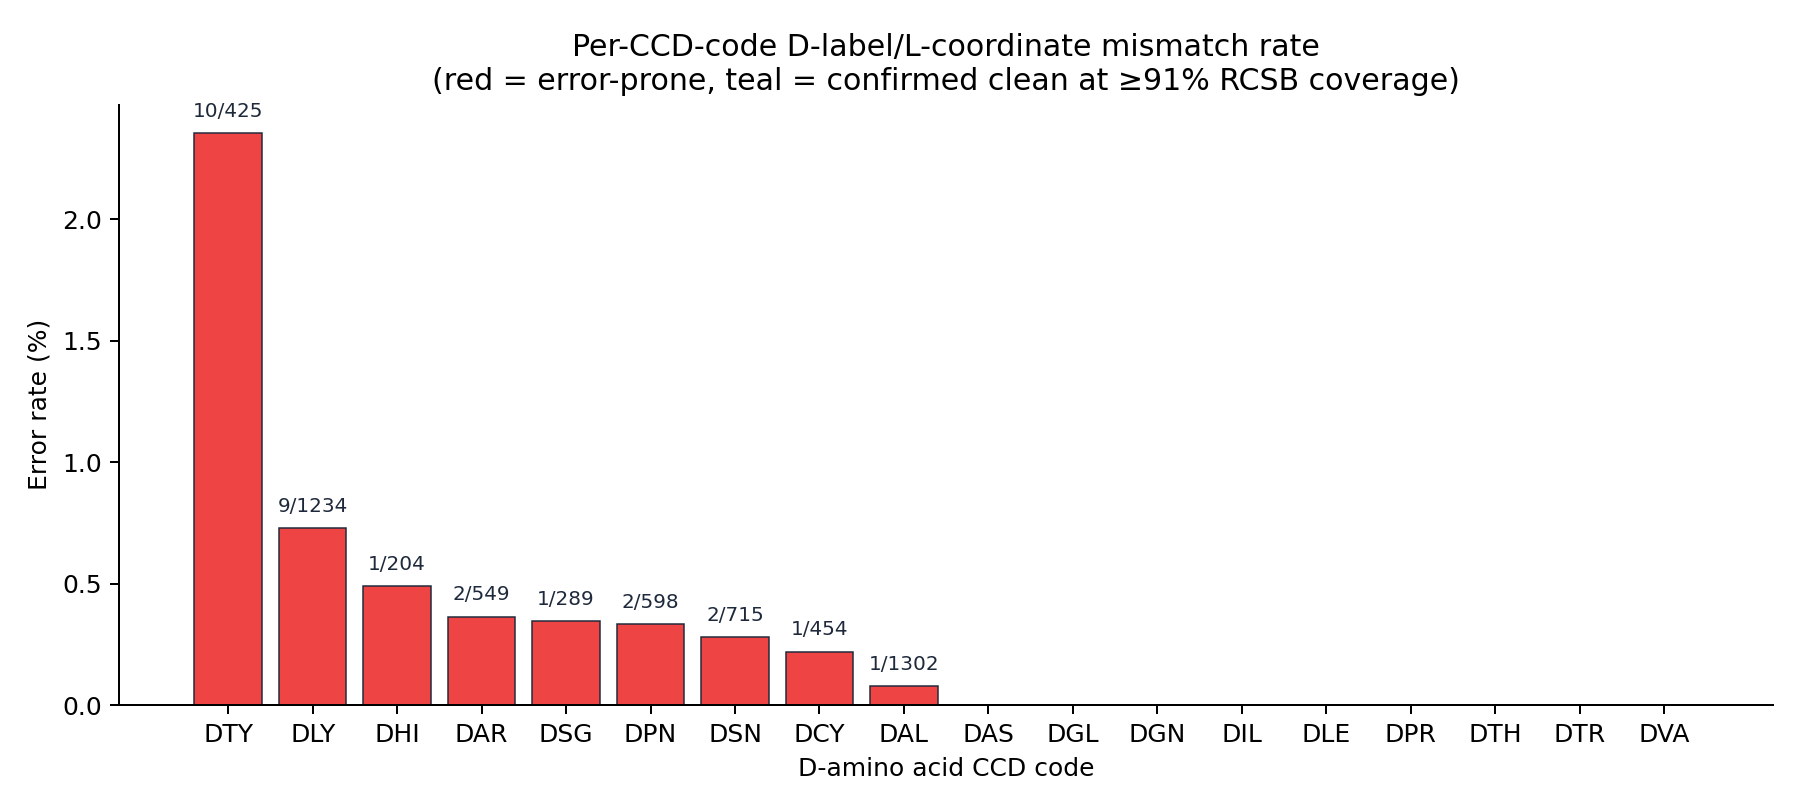
\includegraphics[width=0.95\linewidth]{pdb_survey_figures/fig1_error_rate_per_ccd.png}
\caption{Per-CCD-code error rate across the 18-code survey, sorted by rate. Red bars: error-prone codes ($>0$ errors); teal bars: codes confirmed clean at zero errors. Bar labels show error count / residues checked for error-prone codes.}
\label{fig:err_rate}
\end{figure}

\subsection{Deposition-Year Trend}

In the original 12-structure survey, all error-containing entries were deposited between 1992 and 2005, with deposition year significantly predicting the presence of errors (Mann--Whitney $U=278$, $p=0.0027$). Three further error structures identified in the expanded 4{,}616-file survey were deposited post-remediation: 2RMI (2007), 2W76 (2008), and 3RIT (2011). Figure~\ref{fig:dep_year} plots per-structure error count against deposition year and overlays the 2006--2008 wwPDB remediation window. The persistence of errors after remediation confirms that the deposition pipeline continues to lack a D-specific chirality check. Resolution does not predict errors (Mann--Whitney $U=112$, $p=0.19$); errors span 0.99--3.4~\AA, including the 0.99~\AA\ atomic-resolution 1HHZ case, which carries the largest positive signed volume in the dataset ($+2.70$~\AA$^3$) in a context where D-alanine is a biosynthetic requirement.

\begin{figure}[ht]
\centering
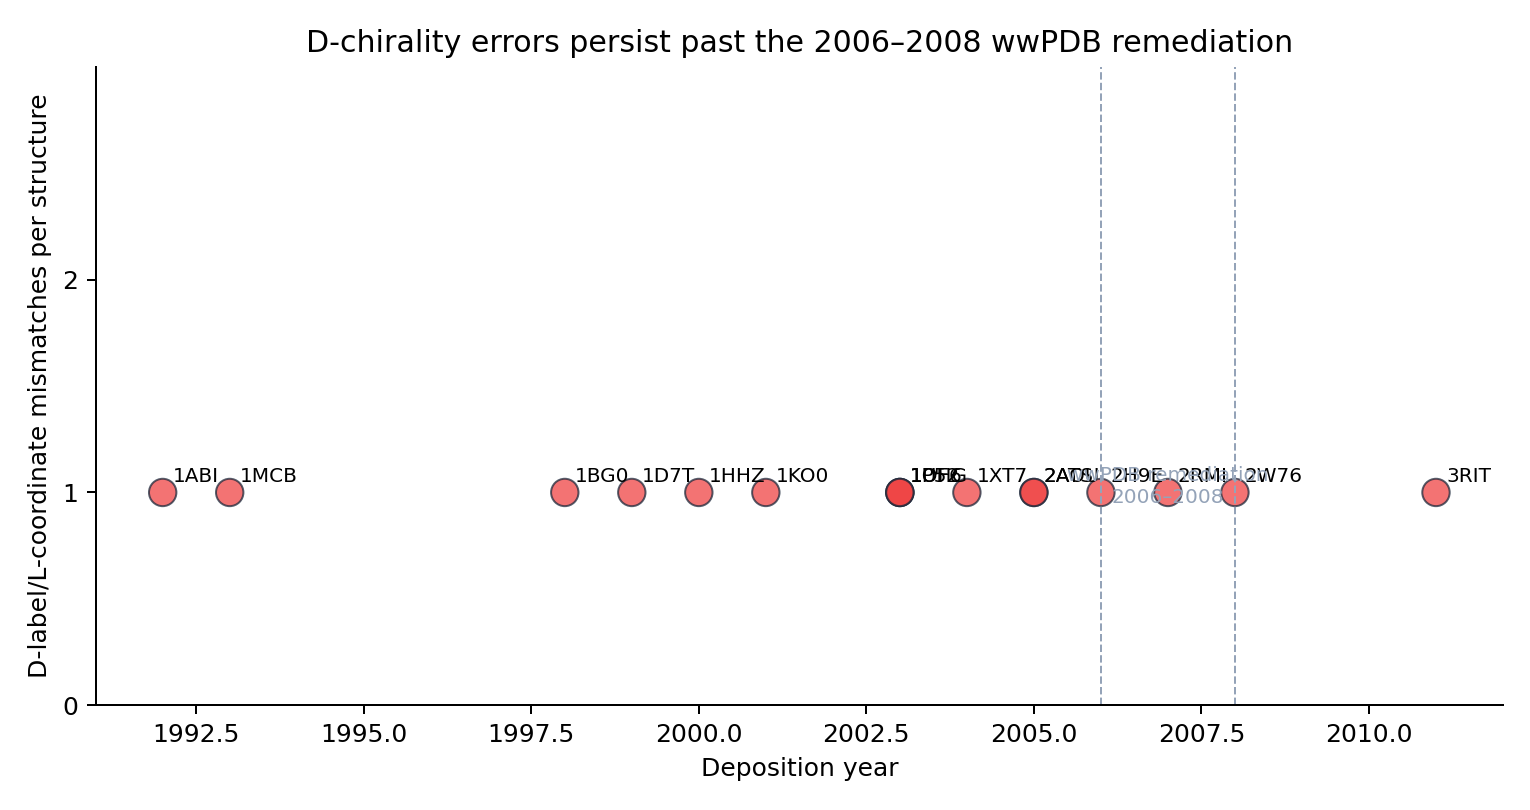
\includegraphics[width=0.95\linewidth]{pdb_survey_figures/fig2_deposition_year_vs_errors.png}
\caption{D-chirality errors persist past the 2006--2008 wwPDB remediation window. Each point is a deposited structure; the y-axis is the number of D-label/L-coordinate mismatches in that structure (point area scales with count). The dashed grey rules mark the start and end of the wwPDB remediation effort.}
\label{fig:dep_year}
\end{figure}

\subsection{Signed-Volume Distribution}

Figure~\ref{fig:sv_dist} shows the distribution of signed volumes across all 12{,}573 D-labeled C$_\alpha$ centers (log-scale y axis). The D-correct distribution clusters cleanly around $-2.5$~\AA$^3$; the 29 mismatches form a tight cluster at $+1.85$ to $+2.77$~\AA$^3$. Two borderline cases sit between the modes at $+0.12$ and $+0.56$~\AA$^3$. The bimodality of the distribution is consistent with the method having a wide unambiguous decision margin between the two configurations.

\begin{figure}[ht]
\centering
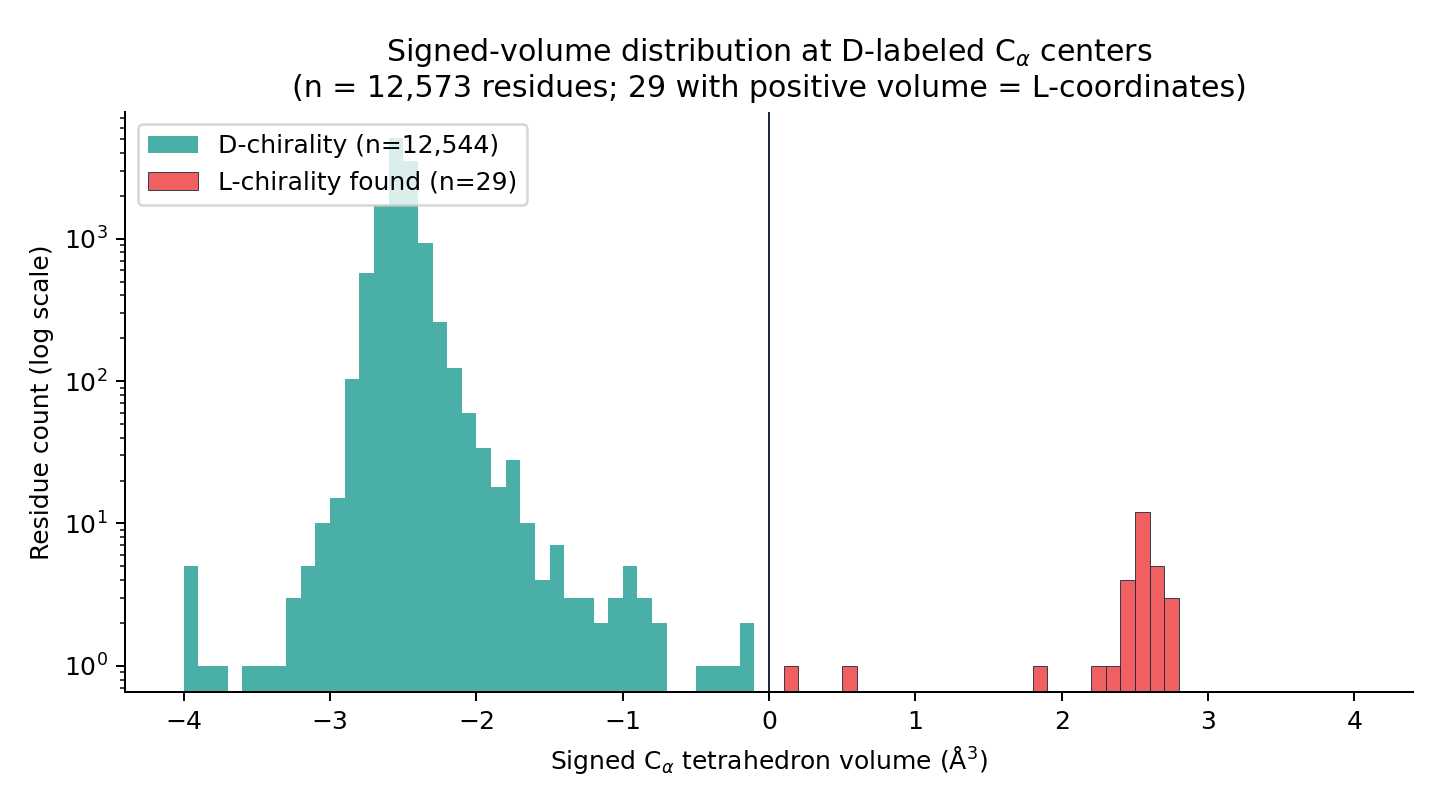
\includegraphics[width=0.95\linewidth]{pdb_survey_figures/fig3_signed_volume_distribution.png}
\caption{Signed-volume distribution at all 12{,}573 D-labeled C$_\alpha$ stereocenters (log-scale y axis). The 29 L-coordinate mismatches form a tight cluster at $+1.85$ to $+2.77$~\AA$^3$, well separated from the $\sim -2.5$~\AA$^3$ D-correct mode.}
\label{fig:sv_dist}
\end{figure}

\section{Discussion}

The 29 mismatches reported here exist along three remediation pathways. The 18 CCD-code misassignments are pure metadata errors: the coordinates are correct, and the fix is to change the three-letter code from the D-form to the L-form (DTY $\to$ TYR, DAR $\to$ ARG, DLY $\to$ LYS). Because the CCD encodes configuration in the InChI \texttt{/m} flag --- L-form codes carry \texttt{/m0} (S-configuration) and D-form codes carry \texttt{/m1} (R-configuration) --- an automated check that computes the signed volume of the ligand from the deposited coordinates and compares it against the \texttt{/m} flag of the selected CCD code would catch every one of these misassignments before the structure enters the archive. The wwPDB \citep{shao2015,outcome2016} already runs similar automated checks for bond-length outliers and geometry; adding a signed-volume-versus-\texttt{/m}-flag cross-validation at deposition is conceptually identical and computationally trivial.

The 6 stereochem and 3 mislabel errors require a different framing. In the stereochem cases, the coordinate error is the finding: in every one of the six structures (antibiotic natural products, engineered peptide toxins, synthetic therapeutic peptides, and a bacterial metabolite), independent biological evidence demands a D-configuration that the deposited coordinates do not realize. These structures were deposited over a thirteen-year window and survived the 2006--2008 remediation effort because that remediation had no D-specific chirality check. The three polymer mislabels are the inverse: standard L-residues annotated with D-amino acid codes, sometimes in the same entry whose COMPND record explicitly specifies L-form.

The 2 borderlines deserve their own category. 1KO0 DLY:542 has a signed volume of $+0.12$~\AA$^3$, lies on alternate conformer B with a $B$-factor of 32.3~\AA$^2$, and was crystallized from a racemic D,L-lysine condition; 2H9E DTY:S:1 has a volume of $+0.56$. Both fall within the regime where electron density may admit either configuration; the method correctly does not commit.

The key practical recommendation is the same for all three remediation pathways: the wwPDB deposition pipeline should validate the configuration of every standard-amino-acid stereocenter against the configuration encoded in the selected CCD code. The check is one cross product, one dot product, and one sign comparison per residue. We provide the reference implementation (\texttt{benchmarks/independent\_d\_residue\_verification.py}) and the complete 12{,}574-row verification dataset alongside this note so that the wwPDB and any third-party validator can reproduce the audit without ChiralFold itself.

\section*{Data Availability}

The full verification dataset is at \url{https://github.com/Tommaso-R-Marena/ChiralFold/blob/master/results/d_residue_verification.csv} (12{,}574 rows including header). Per-error-structure metadata: \url{https://github.com/Tommaso-R-Marena/ChiralFold/blob/master/results/error_table_verified.csv}. CCD-code coverage summary: \url{https://github.com/Tommaso-R-Marena/ChiralFold/blob/master/results/ccd_code_coverage_summary.csv}. Classification JSON: \url{https://github.com/Tommaso-R-Marena/ChiralFold/blob/master/results/error_classification.json}. Independent verification script: \url{https://github.com/Tommaso-R-Marena/ChiralFold/blob/master/benchmarks/independent_d_residue_verification.py}.

\section*{Acknowledgments}

The author thanks the wwPDB consortium for maintaining the Protein Data Bank and the open-source structural biology community.

\section*{Competing Interests}

The author declares no competing interests.

\begin{thebibliography}{9}

\bibitem[Childs et~al.(2025)]{childs2025}
Childs CM, Zhou P, Donald BR.
\newblock Has AlphaFold 3 Solved the Protein Folding Problem for D-Peptides?
\newblock \textit{bioRxiv} 2025.03.14.643307 (2025).
\newblock \href{https://doi.org/10.1101/2025.03.14.643307}{doi:10.1101/2025.03.14.643307}

\bibitem[Chen et~al.(2010)]{chen2010}
Chen VB et~al.
\newblock MolProbity: all-atom structure validation for macromolecular crystallography.
\newblock \textit{Acta Cryst} D66:12--21 (2010).
\newblock \href{https://doi.org/10.1107/S0907444909042073}{doi:10.1107/S0907444909042073}

\bibitem[Lovell et~al.(2003)]{lovell2003}
Lovell SC et~al.
\newblock Structure validation by C$_\alpha$ geometry: $\varphi$,$\psi$ and C$_\beta$ deviation.
\newblock \textit{Proteins} 50:437--450 (2003).
\newblock \href{https://doi.org/10.1002/prot.10286}{doi:10.1002/prot.10286}

\bibitem[Hovm{\"o}ller et~al.(2002)]{hovmoller2002}
Hovm{\"o}ller S, Zhou T, Ohlson T.
\newblock Conformations of amino acids in proteins.
\newblock \textit{Acta Cryst} D58:768--776 (2002).
\newblock \href{https://doi.org/10.1107/S0907444902003359}{doi:10.1107/S0907444902003359}

\bibitem[Henrick et~al.(2008)]{henrick2008}
Henrick K et~al.
\newblock Remediation of the protein data bank archive.
\newblock \textit{Nucleic Acids Res} 36:D426--D433 (2008).
\newblock \href{https://doi.org/10.1093/nar/gkm937}{doi:10.1093/nar/gkm937}

\bibitem[Shao et~al.(2015)]{shao2015}
Shao C et~al.
\newblock The chemical component dictionary: complete descriptions of constituent molecules in experimentally determined 3D macromolecules in the PDB.
\newblock \textit{Bioinformatics} 31:1274--1278 (2015).
\newblock \href{https://doi.org/10.1093/bioinformatics/btu789}{doi:10.1093/bioinformatics/btu789}

\bibitem[Berman et~al.(2016)]{outcome2016}
Berman H et~al.
\newblock Outcome of the First wwPDB/CCDC/D3R Ligand Validation Workshop.
\newblock \textit{Structure} 24:502--508 (2016).
\newblock \href{https://doi.org/10.1016/j.str.2016.02.017}{doi:10.1016/j.str.2016.02.017}

\bibitem[Miyamoto and Homma(2021)]{miyamoto2021}
Miyamoto T, Homma H.
\newblock D-Amino acid metabolism in bacteria.
\newblock \textit{J Biochem} 170:5--13 (2021).
\newblock \href{https://doi.org/10.1093/jb/mvab043}{doi:10.1093/jb/mvab043}

\bibitem[Cava et~al.(2011)]{cava2011}
Cava F et~al.
\newblock Distinct pathways for modification of the bacterial cell wall by non-canonical D-amino acids.
\newblock \textit{EMBO J} 30:3442--3453 (2011).
\newblock \href{https://doi.org/10.1038/emboj.2011.246}{doi:10.1038/emboj.2011.246}

\end{thebibliography}

\end{document}
